\chapter{Interaction discovery for logistic regression} \label{chap5}

\textcolor{red}{needs quote}

\textit{Nota Bene :} Ce chapitre s'inspire fortement ... \textcolor{red}{à adapter au moment de l'envoi du manuscrit}

\selectlanguage{english}

Continuing my pursuit of interpretable representation learning algorithms for logistic regression, I tackle in this chapter a common problem in \textit{Credit Scoring} and other application contexts relying either on logistic regression or additive models of the form $g(y) = \sum_{j=1}^d \theta_j f_j(x_j)$. To further reduce the model bias discussed in Section~\ref{chap1:sec3} and thus obtain better predictive performance while maintaining interpretability, \textit{Credit Scoring} practitioners are used to introducing pairwise interactions.


\section{Motivation}


\section{Pairwise interaction screening as a feature selection problem}


\section{A novel model selection approach}


\section{Discretization and levels merging \textit{with} interactions} \label{sec:discwith}

As described in the introduction, logistic regression is linear in its inputs which does not allow to take into account conditional dependency, see~\cite{berry2010testing}. This problem is often dealt with by sparsely introducing ``interactions'', \textit{i.e.}\ products of two features. Unfortunately, this leads again to a model selection challenge as the number of pairs of features is $\dfrac{d(d-1)}{2}$. We denote by $\bdelta$ the upper triangular matrix with $\delta_{k,\ell} = 1$ if $k < \ell$ and features $k$ and $\ell$ ``interact'' in the logistic regression in the sense of~\cite{berry2010testing}. The logistic regression with interactions $\bdelta$ is thus:
\begin{equation} \label{eq:reglog_sans}
\text{logit}[p_{\glssymbol{bth}}(1|\bm{f}(\bm{x}),\bdelta)] = \theta_{0} + \sum_{j=1}^d \theta_{j}^{f_j(x^j)} + \sum_{1 \leq k < \ell \leq d} \delta_{k,\ell} \theta_{k,\ell}^{f_p(x^p),f_q(x^q)},
\end{equation}
where $\glssymbol{bth} = (\theta_{0},\theta_{1}^1,\dots,\theta_{1}^{m_1},\dots,\theta_{d}^1,\dots,\theta_{d}^{m_d},\theta_{1,2}^{1,1},\dots,\theta_{1,2}^{m_1,m_2},\dots,\theta_{d-1,d}^{1,1},\dots,\theta_{d-1,d}^{m_{d-1},m_d})$ and for all features $j$, $f_j(x_j)=m_j$ is set as the ``reference'' value and consequently for all $j$, $\theta_{j}^{m_j}=0$ and for all $1 \leq k < \ell \leq d$, $\theta_{k,\ell}^{m_k,m_{\ell}}=0$.

\textcolor{red}{eq:criterion undefined = c'est le BIC du chapitre précédent à harmoniser}

\textcolor{red}{sec:discwithout undefined = à reprendre}

Criterion~\eqref{eq:criterion} developed in the context of discretization and grouping can be adapted to take into account interactions
\begin{equation}\label{eq:criterion_inter}
\bm{f}^{\text{opt}},\bdelta^{\text{opt}} = \argmin_{\bm{f},\bdelta} \text{BIC}[p_{\glssymbol{bth}}(\bm{y}|\bm{f}(\bm{x}),\bdelta)].
\end{equation}
The combinatorics involved in this problem are much higher than those of criterion~\eqref{eq:criterion}, which already lead to an untractable greedy approach. For each feasible discretization scheme of Section~\ref{sec:discwithout}, there is now $2^{\frac{d(d-1)}{2}}$ models to test! In the following section, we will first consider the discretization fixed and develop a stochastic approach similar to the one proposed for discretization and grouping of factor levels.

\subsection{With a fixed discretization}

With a fixed discretization scheme $\bm{e} = \bm{f}(\glssymbol{bx})$, criterion~\ref{eq:criterion_inter} amounts to $\bdelta^{\text{opt}} = \argmin_{\bdelta} \text{BIC}[p_{\glssymbol{bth}}(y|\bm{e},\bdelta)]$ which optimization through a greedy approach is untractable with more than a few features ($d > 10$).

Again, $\bdelta$ can be seen as an observation of a latent random matrix and $\bdelta^{\text{opt}}$ can be found using a stochastic approach. The BIC criterion has a desirable property relating it to the posterior probability of the model given the data, \textit{i.e.}\ $p(\bdelta | \be, y) \propto p(y | \be, \bdelta) p(\bdelta) \approx \exp(-\text{BIC}[p_{\glssymbol{bth}}(y|\bm{e},\bdelta)]/2)  p(\bdelta)$. Consequently, one can design an MCMC algorithm like Metropolis-Hastings~\cite{hastings1970monte} which should draw ``good'' interaction matrices $\bdelta$ (\textit{i.e.}\ close to $\bdelta^{\text{opt}}$) from the target distribution $p(\bdelta | \be, y)$.

Metropolis-Hastings only requires a proposal of a transition probability between two states of the Markov chain $q: ({\{0,1\}}^{\frac{d(d-1)}{2}},{\{0,1\}}^{\frac{d(d-1)}{2}}) \mapsto \mathbb{R}$, which would require to compute $2^{d(d-1)}$ probabilities (\textit{i.e.}\ one per unique couple of matrices ($\bdelta^{(1)},\bdelta^{(2)}$)). It is thus desirable to reduce this combinatorics by making further assumptions. In what follows, we restrict possible transitions to matrices that are on a one unit $L^1$ distance to the current interaction matrix, s.t.\ $q(\bdelta^{(1)},\bdelta^{(2)}) = 0$ if $\sum_{k=1}^d \sum_{\ell=1}^d |\delta^{(1)}_{k,\ell} - \delta^{(2)}_{k,\ell}| \neq 1$.

Only $\frac{d(d-1)}{2}$ coefficients are now needed, which can be reinterpreted as the probability to switch on (resp. off) an entry of $\bdelta^{(1)}$ which is currently off (resp. on). We claim that a good intuition about whether two features interact is the relative gain (or loss) in BIC between their bivariate model \textit{with} their interaction and this model \textit{without} their interaction. The rational behind such a procedure is the following: $\forall \: 1 \leq k < \ell \leq d, \; p(\delta_{k,\ell}=1 | e_k, e_{\ell}, y) \propto p_{\glssymbol{bth}}(y | e_k, e_{\ell}, \delta_{k,\ell}=1) p(\delta_{k,\ell}=1) \approx \exp(-\text{BIC}[p_{\glssymbol{bth}}(y | e_k, e_{\ell}, \delta_{k,\ell}=1)]/2) p(\delta_{k,\ell}=1)$. Setting a uniform prior $p(\delta_{k,\ell}=1) =\begin{cases} 0 \text{ if } k \geq \ell \\ \frac{1}{2} \text{ otherwise.} \end{cases}$ and writing the same expression for $\delta_{k,\ell} = 0$ yields: $p_{k,\ell} = p(\delta_{k,\ell}=1 | e_k, e_{\ell}, y) \approx \exp \left( \frac{\text{BIC}[p_{\glssymbol{bth}}(y | e_k, e_{\ell}, \delta_{k,\ell}=0)]-\text{BIC}[p_{\glssymbol{bth}}(y | e_k, e_{\ell}, \delta_{k,\ell}=1)]}{2} \right)$. We normalize $p_{k,\ell}$ s.t.\ $\sum_{1 \leq k < \ell \leq d} p_{k,\ell} = 1$.

We claim that if $p_{k,\ell}$ is close to $1$ (resp. $0$), then there is a strong chance that $\delta_{k,\ell}^\star = 1$ (resp. $\delta_{k,\ell}^\star = 0$) even in the full multivariate model, which is in particular true if features $e_k$ and $e_{\ell}$ are independent to other features $e_r$, $r \neq k$, $r \neq \ell$. Consequently, if at step $(s)$ of the Markov chain, $\delta_{k,\ell}^{(s)} = 1$ (resp. $0$) and $p_{k,\ell}$ is close to $0$ (resp. $1$), a good candidate for $\bdelta^{(s+1)}$ should be to change $\delta_{k,\ell}$ to $\delta_{k,\ell}^{(s+1)} = 0$ (resp. $\delta_{k,\ell}^{(s+1)} = 1$). Our proposal is thus to calculate the difference between the current interaction matrix and $(p_{k,\ell})_{1 \leq k,\ell, \leq d}$ which we denote by $q_{k,\ell}^{(s)} = |\delta_{k,\ell}^{(s)} - p_{k,\ell}|$ and normalize. This defines a proper transition probability between two interaction matrices: $q(\bdelta^{(s)},\bdelta') = \begin{cases} 0 \text{ if } \sum_{k=1}^d \sum_{\ell=1}^d |\delta^{(s)}_{k,\ell} - \delta_{k,\ell}'| \neq 1, \\ q_{k,\ell}^{(s)} \text{ for the unique couple } (k,\ell) \text{ s.t.} \: \delta^{(s)}_{k,\ell} \neq \delta_{k,\ell}'. \end{cases}$

Now, a Metropolis-Hastings step can be conducted by drawing $\bdelta' \sim q(\bdelta^{(s)},\cdot)$. The acceptance probability of this candidate is given by $\alpha = \min \left( 1, \frac{p(\bdelta' | \be,y)}{p(\bdelta^{(s)} | \be, y)} \frac{1-q(\bdelta^{(s)},\bdelta')}{q(\bdelta^{(s)},\bdelta')} \right) \approx \min \left( 1, \exp \left( \frac{\text{BIC}[p_{\glssymbol{bth}}(y | \be, \bdelta^{(s)})] - \text{BIC}[p_{\glssymbol{bth}}(y | \be, \bdelta')]}{2} \right) \frac{1-q(\bdelta^{(s)},\bdelta')}{q(\bdelta^{(s)},\bdelta')} \right)$. If $\alpha \geq 1$, the candidate is accepted and $\bdelta^{(s+1)} = \bdelta'$; otherwise, the candidate is accepted with probability $\alpha$ s.t.\ $\bdelta^{(s+1)} = \begin{cases} \bdelta' \text{ with probability } \alpha, \\ \bdelta^{(s)} \text{ with probability } 1-\alpha. \end{cases}$

The existence of the stationary distribution $p(\bdelta | \be,y)$ is guaranteed by construction of the Metropolis-Hastings algorithm as the generated Markov chain fulfills the detailed balance condition. The uniqueness of the stationary distribution is given by the ergodicity of the Markov chain: as $\forall \: 1 \leq  k < \ell \leq d, \: q_{k,\ell} > 0$ and a transition changes only one entry $\delta_{k,\ell}$ of the interaction matrix, every state can be reached in at most $\frac{d(d-1)}{2}$ steps.

In practice with a fixed discretization scheme, this stochastic approach is probably outperformed in computing time by Lasso-based methods or correlation-based methods like~\cite{simon}, which might obtain a suboptimal model in a fixed computing time, contrary to our approach which might take lots of steps to converge in distribution. Its double benefit however lies in the ability of the practitioner to define before-hand how many steps shall be performed and the natural integration to the discretization and grouping of factor levels algorithm proposed in the previous section, which we develop in the next one.

\subsection{While discretizing and grouping}

Quand on connaît $\delta$, on tire $E$ comme avant.

Quand on connaît $E$, on tire $\delta$ comme montré ci-dessus.

L'algorithme de Gibbs fonctionne comme ça.

\subsection{Experiments on simulated data \textit{with} interactions}

\subsubsection{With a fixed discretization}





\subsubsection{While discretizing and grouping}

\begin{figure}
\centering
\resizebox{\linewidth}{6cm}{%
% Created by tikzDevice version 0.11 on 2018-07-20 11:37:01
% !TEX encoding = UTF-8 Unicode
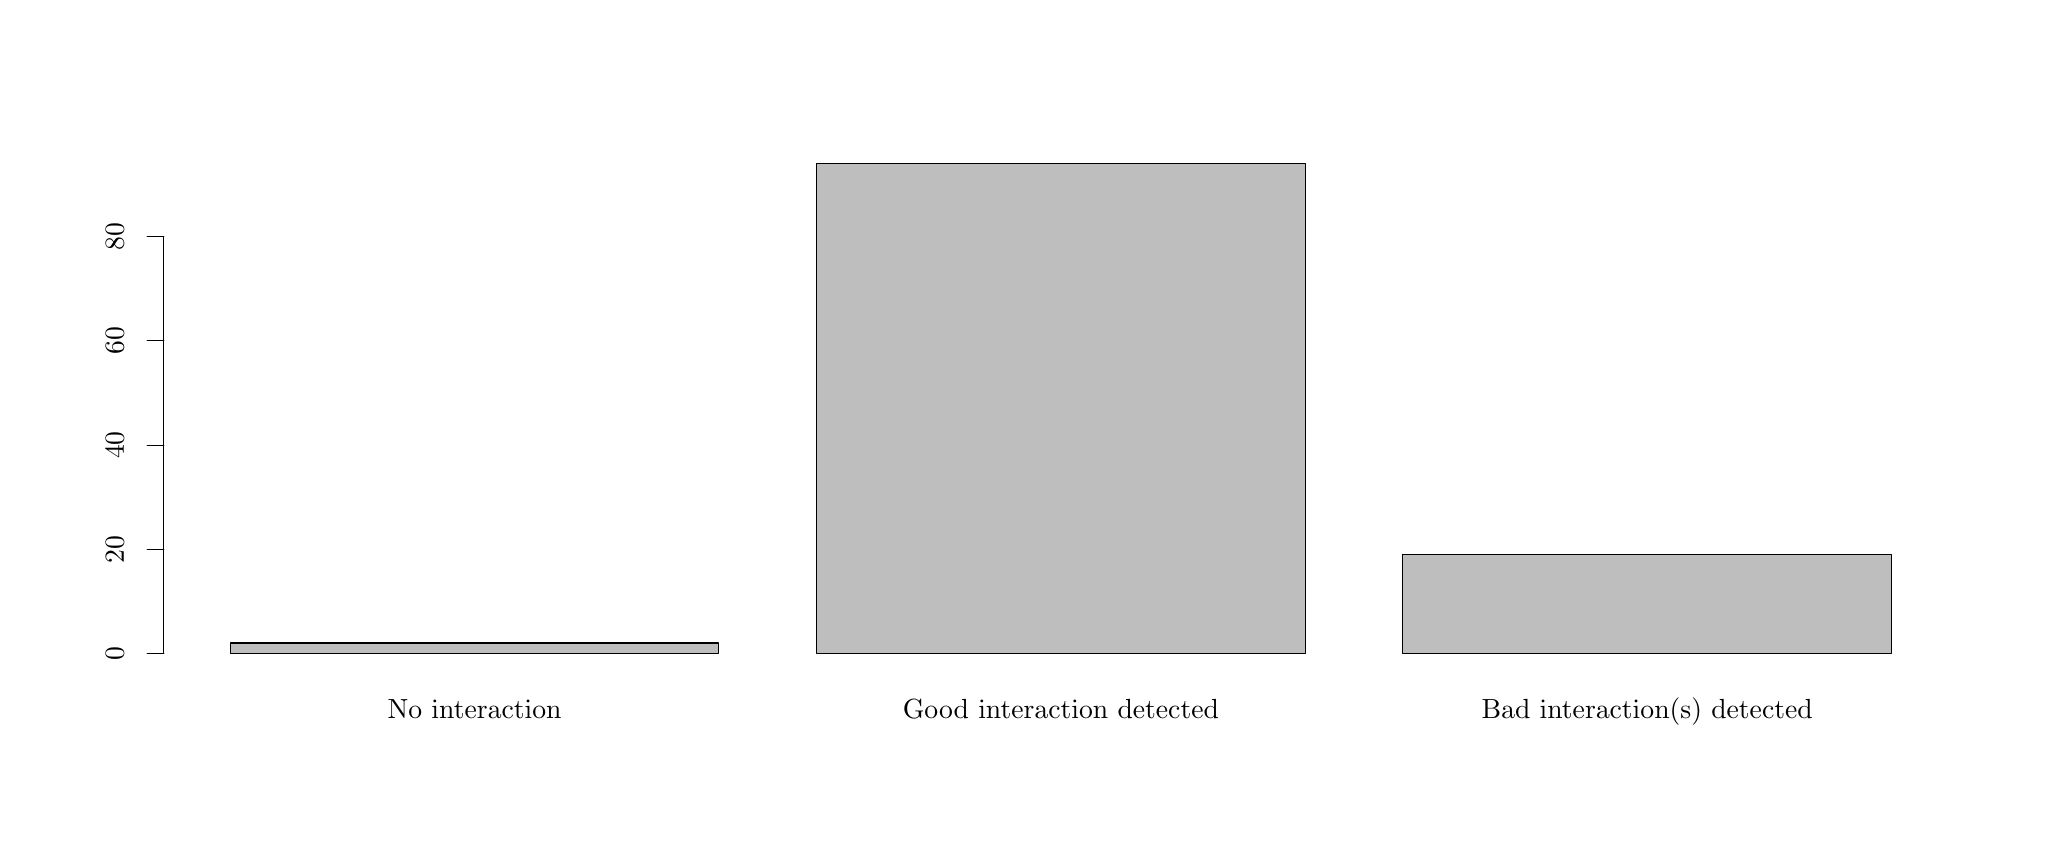
\begin{tikzpicture}[x=1pt,y=1pt]
\definecolor{fillColor}{RGB}{255,255,255}
\path[use as bounding box,fill=fillColor,fill opacity=0.00] (0,0) rectangle (722.70,289.08);
\begin{scope}
\path[clip] (  0.00,  0.00) rectangle (722.70,289.08);
\definecolor{drawColor}{RGB}{0,0,0}
\definecolor{fillColor}{RGB}{190,190,190}

\path[draw=drawColor,line width= 0.4pt,line join=round,line cap=round,fill=fillColor] ( 73.21, 62.97) rectangle (249.76, 66.73);

\path[draw=drawColor,line width= 0.4pt,line join=round,line cap=round,fill=fillColor] (285.07, 62.97) rectangle (461.63,239.88);

\path[draw=drawColor,line width= 0.4pt,line join=round,line cap=round,fill=fillColor] (496.94, 62.97) rectangle (673.49, 98.73);
\end{scope}
\begin{scope}
\path[clip] (  0.00,  0.00) rectangle (722.70,289.08);
\definecolor{drawColor}{RGB}{0,0,0}

\node[text=drawColor,anchor=base,inner sep=0pt, outer sep=0pt, scale=  1.00] at (161.49, 39.60) {No interaction};

\node[text=drawColor,anchor=base,inner sep=0pt, outer sep=0pt, scale=  1.00] at (373.35, 39.60) {Good interaction detected};

\node[text=drawColor,anchor=base,inner sep=0pt, outer sep=0pt, scale=  1.00] at (585.21, 39.60) {Bad interaction(s) detected};

\path[draw=drawColor,line width= 0.4pt,line join=round,line cap=round] ( 49.20, 62.97) -- ( 49.20,213.53);

\path[draw=drawColor,line width= 0.4pt,line join=round,line cap=round] ( 49.20, 62.97) -- ( 43.20, 62.97);

\path[draw=drawColor,line width= 0.4pt,line join=round,line cap=round] ( 49.20,100.61) -- ( 43.20,100.61);

\path[draw=drawColor,line width= 0.4pt,line join=round,line cap=round] ( 49.20,138.25) -- ( 43.20,138.25);

\path[draw=drawColor,line width= 0.4pt,line join=round,line cap=round] ( 49.20,175.89) -- ( 43.20,175.89);

\path[draw=drawColor,line width= 0.4pt,line join=round,line cap=round] ( 49.20,213.53) -- ( 43.20,213.53);

\node[text=drawColor,rotate= 90.00,anchor=base,inner sep=0pt, outer sep=0pt, scale=  1.00] at ( 34.80, 62.97) {0};

\node[text=drawColor,rotate= 90.00,anchor=base,inner sep=0pt, outer sep=0pt, scale=  1.00] at ( 34.80,100.61) {20};

\node[text=drawColor,rotate= 90.00,anchor=base,inner sep=0pt, outer sep=0pt, scale=  1.00] at ( 34.80,138.25) {40};

\node[text=drawColor,rotate= 90.00,anchor=base,inner sep=0pt, outer sep=0pt, scale=  1.00] at ( 34.80,175.89) {60};

\node[text=drawColor,rotate= 90.00,anchor=base,inner sep=0pt, outer sep=0pt, scale=  1.00] at ( 34.80,213.53) {80};
\end{scope}
\end{tikzpicture}

}
\caption{\label{fig:simulated_interaction}Distribution of the kind of interactions chosen by \textit{glmdisc} on 100 simulations.}
\end{figure}


\section{Benchmark of \textit{glmdisc} against other approaches} \label{sec:exp}

\subsection{Simulated data from a misspecifed model}

\subsection{Real data from Crédit Agricole Consumer Finance}

\section{Conclusion} \label{sec:ccl}

The essentially industrial problem of discretization, grouping of factor levels and introduction of interactions in a supervised multivariate classification setting was formalized and a new approach, named \textit{glmdisc} has been proposed.

This algorithm relies on the use of logistic regression, although other predictive models can be plugged in place of $p_{\glssymbol{bth}}$. Similarly, our proposed use of polytomous logistic links between each discretized feature and their respective continuous version can be replaced by any other univariate multiclass predictive model, which makes it flexible and adaptable to other problems.

The experiments showed that, as was sensed empirically by statisticians in the field of \textit{Credit Scoring}, discretization, grouping and interactions can indeed provide better models than standard logistic regression. This novel approach allows practitioners to have a fully automized and statistically well-grounded tool that achieves better performance than both \textit{ad hoc} industrial practices and academic discretization heuristics at the price of decent computing time but much less of the practitioner's valuable time.

The code used for numerical experiments is available as packages, in the \textsf{R} programming language on CRAN and in the Python programming language on PyPi. Both packages are named \textit{glmdisc}. \textcolor{red}{à modifier}














\printbibliography[heading=subbibliography, title=References of Chapter 4]
